\documentclass{article}
\usepackage[a4paper,
            left=1in,
            right=1in,
            top=1in,
            bottom=1in]{geometry}
\usepackage[T1]{fontenc}
\usepackage[polish]{babel}
\usepackage[utf8]{inputenc}
\usepackage{lmodern}
\usepackage{listings}
\usepackage{graphicx}
\usepackage{color}

\title{Gra w życie}
\author{Oleksii Yermolaiev, grupa 16c}

\definecolor{comment}{RGB}{0,128,0}
\definecolor{string}{RGB}{255,0,0}
\definecolor{keyword}{RGB}{0,0,255}

\lstset{
    language=Python,
    literate={Ć}{{\'C}}1 {ć}{{\'c}}1
             {Ś}{{\'S}}1 {ś}{{\'s}}1
             {Ó}{{\'O}}1 {ó}{{\'o}}1
             {Ź}{{\'Z}}1 {ź}{{\'z}}1
             {Ż}{{\.Z}}1 {ż}{{\.z}}1
             {Ą}{{\k A}}1 {ą}{{\k a}}1
             {Ę}{{\k E}}1 {ę}{{\k e}}1
             {Ń}{{\'N}}1 {ń}{{\'n}}1
             {Ł}{{\L}}1 {ł}{{\l}}1,
    frame=single,
    showstringspaces=false,
    numbers=left,
    tabsize=4,
    title=\lstname,
    basicstyle=\ttfamily\small,
    numberstyle=\footnotesize,
    commentstyle=\color{comment},
    stringstyle=\color{string},
    keywordstyle=\color{keyword},
}

\begin{document}

\maketitle

\section{Opis projektu}

Prosta symulacja gry w życie z możliwością zmiany reguł.

\begin{figure}[h]
\centering
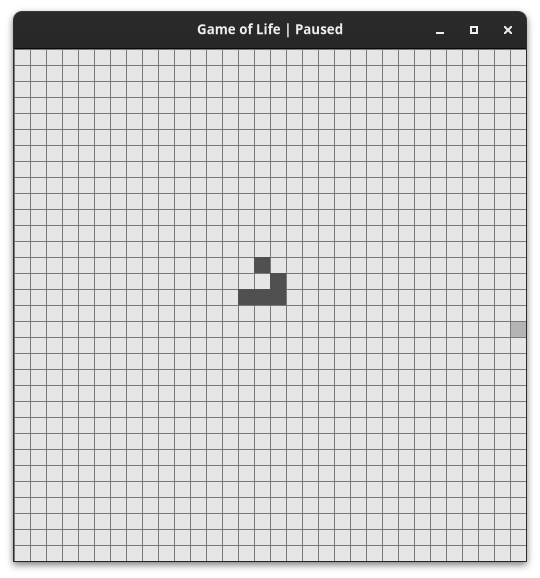
\includegraphics[width=200pt]{screenshots/glider.png}
\caption{Klasyczny ``Glider''.}
\end{figure}

\subsection{Sterowanie}
\begin{itemize}
  \item Kiedy symulacja aktywna:
    \begin{itemize}
      \item \texttt{LPM} --- ustaw żywą komórkę;
      \item \texttt{PPM} --- ustaw martwą komórkę;
    \end{itemize}
  \item Przełączenie trybów:
    \begin{itemize}
      \item \texttt{escape} --- zmień reguły;
      \item \texttt{spacja} --- zatrzymaj, kontynuuj;
    \end{itemize}
  \item Kiedy zatrzymano:
    \begin{itemize}
      \item \texttt{enter}  --- zrób jeden krok.
    \end{itemize}
\end{itemize}

\subsection{Reguły}

Przy każdym kroku gry dla każdej komórki:
\begin{itemize}
  \item Jeżeli jest żywa, regułę określa wierzchni rząd przełączników;
  \item Jeżeli jest martwa, regułę określa dolny rząd przełączników;
\end{itemize}
Nowy stan komórki określa $n$ty przęłącznik rzędu, gdzie $n$ - liczba jej żywych sąsiadów.
\begin{itemize}
  \item Jeżeli jest włączony, komórka żyje;
  \item Jeżeli jest wyłączony, komórka nie żyje.
\end{itemize}

\begin{figure}[h]
\centering
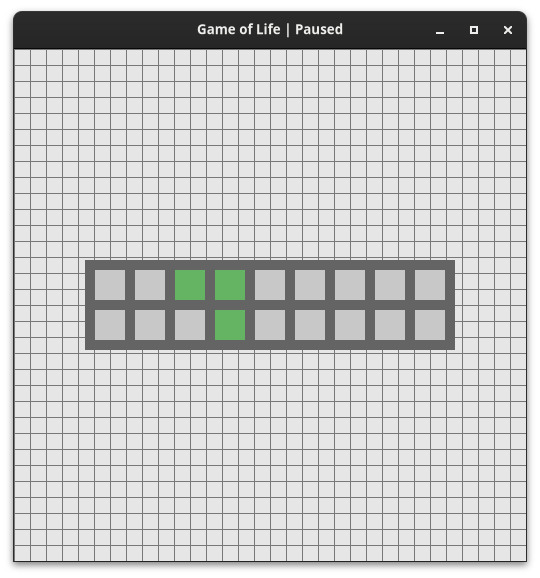
\includegraphics[width=200pt]{screenshots/rules.png}
\caption{Menu zmiany reguł.}
\end{figure}

\section{Opis procesu projektowania}
Zacząłem od kodu jednego z zadań domowych z PSM. Rozdzieliłem kod na kilka plików,
bo stawał się zbyt długi oraz użyłem klas dla lepszej czytelności. Dodałem graficzne menu
dla zmiany reguł, zmieniłem reprezentację wewnętrzną reguł dla optymalizacji.

\subsection{Podział ról w zespole}
Wszystko zrobiłem samemu.

\section{Podsumowanie}
Python jest fajnym językiem dla małych programów. Mi się spodobała praca nad projektem
i wynik moich starań.

\pagebreak

\section{Kod projektu}
\lstinputlisting{src/main.py}
\lstinputlisting{src/game.py}
\lstinputlisting{src/menu.py}
\lstinputlisting{src/gui.py}

\end{document}
